\documentclass[11pt]{article}

\hoffset        2mm 
\voffset        -15mm
\oddsidemargin  0mm
\topmargin      0.5in
\textwidth      6in
\textheight     9in

\usepackage{graphicx,amsmath, amssymb, amsthm, amsfonts}


% Define the theorem styles and numbering
\theoremstyle{plain}
\newtheorem{theorem}{Theorem}[section] % changed counter "chapter" to "section" for use in an article
\newtheorem{proposition}[theorem]{Proposition}
\newtheorem{corollary}[theorem]{Corollary}
\newtheorem{lemma}[theorem]{Lemma}

\theoremstyle{definition}
\newtheorem{definition}[theorem]{Definition}
\newtheorem{example}[theorem]{Example}

\theoremstyle{remark}
\newtheorem*{remark}{Remark}
\newtheorem*{claim}{Claim}




%% Create shortcut commands for various fonts and common symbols
%\newcommand{\k}{\kappa}
\newcommand{\C}{\mathbb{C}}
\newcommand{\veps}{\varepsilon}
\newcommand{\eps}{\epsilon}
\newcommand{\f}{\textbf{f}}
\newcommand{\fb}{\textbf{f}}
\newcommand{\F}{\mathbb{F}}
\newcommand{\Fb}{\textbf{F}}
\newcommand{\gb}{\textbf{g}}
\newcommand{\h}{\textbf{h}}
\newcommand{\kb}{\textbf{k}}
\newcommand{\M}{\mathcal{M}}
\newcommand{\N}{\mathbb{N}}
\newcommand{\Norm}{\textbf{N}}
\newcommand{\n}{\textbf{n}}
\newcommand{\vp}{\varphi}
\newcommand{\vph}{\hat{\varphi}}
\newcommand{\p}{\phi}
% note:  \P is already defined to be the paragraph symbol
\newcommand{\Proj}{\mathbb{P}}
\newcommand{\Pcal}{\mathcal{P}}
\newcommand{\Q}{\mathbb{Q}}
\newcommand{\R}{\mathbb{R}}
\newcommand{\rb}{\textbf{r}}
\newcommand{\s}[1]{\mathcal{#1}}
\newcommand{\supp}{\text{supp}}
\newcommand{\Surf}{\textbf{S}}
\newcommand{\tpsi}{\tilde{\psi}}
\newcommand{\ub}{\textbf{u}}
\newcommand{\U}{\textbf{U}}
\newcommand{\vb}{\textbf{v}}
\newcommand{\V}{\mathbb{V}}
\newcommand{\wb}{\textbf{w}}
\newcommand{\x}{\textbf{x}}
\newcommand{\xh}{\hat{x}}
\newcommand{\X}{\textbf{X}}
\newcommand{\y}{\textbf{y}}
\newcommand{\yh}{\hat{y}}
\newcommand{\Y}{\textbf{Y}}
\newcommand{\Z}{\mathbb{Z}}


%% Declare custom math operators
\DeclareMathOperator{\sech}{sech}
\DeclareMathOperator{\atanh}{atanh}
\DeclareMathOperator{\sign}{sign}
\DeclareMathOperator{\tr}{Trace}
\DeclareMathOperator{\gradsymm}{\nabla_{s}}
\DeclareMathOperator{\divergence}{div}
\DeclareMathOperator{\diag}{diag}
\DeclareMathOperator*{\argmin}{argmin}
\DeclareMathOperator*{\argmax}{argmax}
\DeclareMathOperator{\Span}{Span}
\DeclareMathOperator{\rank}{rank}


%% Sets and systems
\newcommand{\br}[1]{\left\langle #1 \right\rangle}
\newcommand{\paren}[1]{\left(#1\right)}
\newcommand{\sq}[1]{\left[#1\right]}
\newcommand{\set}[1]{\left\{\: #1 \:\right\}}
\newcommand{\setp}[2]{\left\{\, #1\: \middle|\: #2 \, \right\}}
\newcommand{\abs}[1]{\left| #1 \right|}
\newcommand{\norm}[1]{\left\| #1 \right\|}
\newcommand{\system}[1]{\left\{ \begin{array}{rl} #1 \end{array} \right.}

\newcommand{\pf}[2]{\frac{\partial #1}{\partial #2}}
\newcommand{\ipt}[2]{\langle #1,#2 \rangle}
\newcommand{\ip}{\int_{-\infty}^{+\infty}}

\renewcommand{\ker}[1]{\mathcal{N}(#1)}
\newcommand{\ran}[1]{\mathcal{R}(#1)}

%% referencing commands
\newcommand{\thmref}[1]{Theorem \ref{#1}}
\newcommand{\corref}[1]{Corollary \ref{#1}}
\newcommand{\lemref}[1]{Lemma \ref{#1}}
\newcommand{\propref}[1]{Proposition \ref{#1}}
\newcommand{\defref}[1]{Definition \ref{#1}}
\newcommand{\exampleref}[1]{Example \ref{#1}}
\newcommand{\exerref}[1]{Exercise \ref{#1}}

% set the labeling style
\renewcommand{\labelenumi}{(\roman{enumi})} % handy file (include.tex) for all your special commands.  must be in same directory as this .tex file
\graphicspath{{./Figures/}} % folder that will contain all your figures that you want to include.  Must be in same directory as this .tex file



\begin{document}
	
	\ifpdf
	\DeclareGraphicsExtensions{.pdf, .jpg, .tif, .png}
	\else
	\DeclareGraphicsExtensions{.eps, .jpg, .png}
	\fi

\begin{titlepage}

\vspace*{55mm}
\begin{center}
{\huge MATH610-600}\\[1cm]
{\em \huge Programming Assignment \#1}\\[70mm]
{\large February 1, 2012} \\[15mm]
\end{center}

\begin{flushright}
{\LARGE YOUR NAME}
\end{flushright}

\vfill

\end{titlepage}

\newpage
\section{Problem Specifications}
In this section you should describe the problems in this particular assignment.
I would use a separate subsection for describing each problem.
\subsection{Problem 1 (Deflection of a uniformly loaded plate)}
Here we describe what the first problem in this assignment asks us to do.
\subsection{Problem 2 (...)}
Here we describe what the second problem in this assignment asks us to do.

\section{Preliminaries}
In this section you should describe your approach to solving the problems
in this example. You do NOT need to include the source code for your 
programs in your report. If you feel that you should include some \textbf{small}
parts of the code in order to explain things better, you may do it like
this:
\begin{verbatim}
//This function calculates the factorial (n!) of an integer n>=0
//using a 'for' loop in C++
unsigned int factorial(unsigned int n)
{
  unsigned int i, result = 1;
  
  for(i=1; i<=n; i++)
    result *= i;

  return result;
}
\end{verbatim}

To show a table of results that demonstrates some order of convergence,  you can set up a table like Table~\ref{table:ErrorRatesForTimeDependentProblem} that will display the results in an easy to read format

\begin{table}[h!]
\begin{center}
\begin{tabular}{|c|c|c|c|c|c|c|} 
	\hline
cycle & dt & n\_dt's & n\_dofs & h & $\|u_h-u\|_{L^{\infty}([0,T];L^2(\Omega))}$ & $L^{\infty}([0,T];L^2(\Omega))$ rate \\ \hline
     0 & 2.5000e-03   &   80  &  1089  &  6.2500e-02   &  4.4741e-04     &   0.0000 \\
     1 & 1.2500e-03   &  160  &  4225  &  3.1250e-02   &  1.0195e-04     &   2.1337 \\
     2 & 6.2500e-04   &  320  & 16641  &  1.5625e-02   &  2.4712e-05     &   2.0447 \\
     3 & 3.1250e-04   &  640  & 66049  &  7.8125e-03   &  6.0788e-06     &   2.0233 \\ \hline
\end{tabular}
\end{center}
	\caption{Time Convergence results using Runge-Kutta 2 (RK2) algorithm for time discretization using the $\|u_h-u\|_{L^{\infty}([0,T];L^2(\Omega))} = \max_{t\in[0,T]} \|u_h(t)-u(t)\|_{L^2(\Omega)}$ norm.  We expect to see order 2 convergence for small enough mesh size which is confirmed above by experiment.}
	\label{table:ErrorRatesForTimeDependentProblem}
\end{table}


To insert a figure we can put it next and reference it as Figure~\ref{fig:conv_rates_LinfL2} like this.
\begin{figure}[h!]
	\centering
		 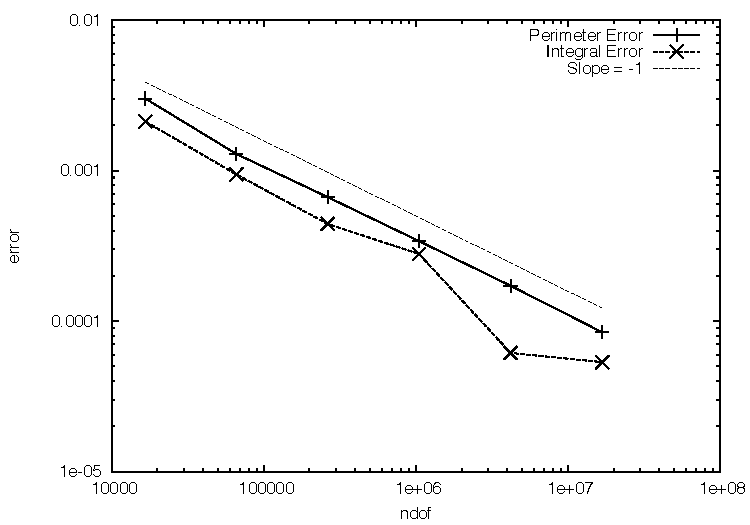
\includegraphics[scale=1.0]{levelset_convergence_rate}
	 	\caption{The log-log plot of our approximation of the integral around $\Gamma$ by using a smeared Dirac delta function of width h.  The reproted values are the errors for perimeter or length $|\Gamma|$ given by $|\int_{\Gamma}ds - \int_{\Omega}\delta_{h}|\nabla\varphi|d\x|$ and the errors for the integral of a function $f(\x)$ defined on $\Gamma$ given by $|\int_{\Gamma}fds - \int_{\Omega}f(\x)\delta_{h}(\x)|\nabla\varphi|d\x|$ plotted against the number of degrees of freedom of our system.  For uniform mesh, we have $h \approx 1/N^d$ where we have N degrees of freedom.}
  \label{fig:conv_rates_LinfL2}
\end{figure}

\newpage

\section{Problem 1(...)}
Give the results and a small discussion of the results that you obtained.

{\bf NOTE:} If you prefer, you may do so in 
a separate subsection for each particular problem.

\section{Problem 2 (...)}
Give the results and a small discussion of the results that you obtained.

\end{document}








